\section{Temporal Perspectives of Honey Bee Networks}
\label{sec:temporalresults}
I investigate the stability of local and global properties, as well as the stability of age and spatial distribution of functional groups of bees.
Furthermore, the dynamics of individual bees' group membership over time are examined.

For all three snapshots, the same link weights distribution can be seen in Figure~\ref{fig:123edges}.
The analysis of snapshot~1 and~2 showed that the same characteristic distribution of degree, strength, lcc, betweenness, and closeness for snapshot~1~(Figure~\ref{fig:n1-degreeStrLCC}) and snapshot~2~(Figure~\ref{fig:n2-degreeStrLCC}) exists. They also follow a normal distribution. The correlation between the local measure and detection frequency and age remains.
All of this shows that the characteristics described in Section~\ref{subsubsec:bees} apply for all three snapshots and are therefore stable for the investigated time interval. A low hierarchical structure and the correlation with age and detection frequency seem to be global properties of the colony.

%%%%%%%%%%%%%%%%%%%%%%%%%%%%%%%%%%%%%%%%%%%%%%%%%%%%%%%%%%%%%%%%%%%%%%%%%%%%%%%
\subsection{Stability of Functional Groups}
%%%%%%%%%%%%%%%%%%%%%%%%%%%%%%%%%%%%%%%%%%%%%%%%%%%%%%%%%%%%%%%%%%%%%%%%%%%%%%%
Table~\ref{tab:communities} lists the exact number of bees per community for each algorithm and snapshot.
For each snapshot, LE detected two communities with about the same number of bees.
The first communities CY(1,2,3) contain the queen and on average younger bees than the second communities CO(1,2,3).

In comparison, WT identified three communities in snapshot~2 and~3 but only two communities in snapshot~1.
The first communities CY(1,2,3) consist of the queen and on average younger bees than the second CM(2,3) and third communities CO(1,2,3).
The bees in CM2 and CM3 are on average younger than the bees in CO2 and CO3.
Figure~\ref{fig:ageDistLE} and~\ref{fig:ageDistWT} depicts the age distribution for each community and snapshot.

A two-sample Kolmogorov–Smirnov test showed that the age distributions are significantly different~($p< 0.001$) for both algorithms.
The spatial segregation of the communities is very similar in all three snapshots. For further reference see the heat maps in~\ref{fig:communitiesPerNetworkWT} and~\ref{fig:communitiesPerNetworkLE}.
The detected communities seem to differ in their respective age and occupy different areas of the comb, but remain stable over this inpected time interval.

\begin{table}
\centering
\caption[Overview about communities]{\textbf{Overview about communities per network} Communities marked with * contain the queen. Age and standard deviation (SD) are measured in days. For each network the queen and bees with a negative agre are excluded: network 1 - 12 bees, network 2 - 119 bees, network 3 - 10 bees.}
\label{tab:communities}
\vspace*{5mm}
\begin{tabular}{lcrrrrr}
	\toprule
	{}  & ID & Members & Proportion & Age & SD\\
	\midrule
	\rowcolor{Gray}
	Leading eigenvector &&&&&\\
	\midrule 
	\quad Network 1  & CY1 & $*430$  & 47.25\% & $17.12$ & $\pm10.97$ \\
	                 & CO1 & $480$   & 52.75\% & $27.24$ & $\pm10.96$ \\
	\midrule   							
	\quad Network 2  & CY2 & $*392$  & 45.63\% & $20.24$ & $\pm12.01$ \\
	                 & CO2 & $467$   & 54.37\% & $28.10$ & $\pm10.88$ \\
	\midrule  
	\quad Network 3  & CY3 & $*381$  & 41.78\% & $13.15$ & $\pm13.50$ \\
	                 & CO3 & $531$   & 58.22\% & $28.70$ & $\pm11.67$ \\
    \midrule
    \rowcolor{Gray}
    Walktrap &&&&&\\
    \midrule 
	\quad Network 1 & CY1 & $*427$ & 46.92\% & $17.07$ & $\pm10.92$\\
	                & CO1 & $482$  & 52.97\% & $27.23$ & $\pm11.00$\\
	\midrule
	\quad Network 2 & CY2 & $*263$ & 30.62\% & $18.23$ & $\pm11.46$\\
				    & CM2 & $305$  & 35.51\% & $25.20$ & $\pm11.47$\\
				    & CO2 & $291$  & 33.88\% & $29.47$ & $\pm10.06$\\            
	\midrule
	\quad Network 3 & CY3 & $*229$  & 25.11\% & $6.55$  & $\pm10.36$\\
					& CM3 & $298$  & 32.68\% & $25.08$ & $\pm11.97$\\
					& CO3 & $385$  & 42.21\% & $29.29$ & $\pm11.44$\\
	\bottomrule
\end{tabular}
\end{table}
\begin{table}
\centering
\caption[Kolmogorov-Smirnov test]{\textbf{Kolmogorov-Smirnov test} $p$-values for leading eigenvector (LE) and walktrap (WT) for each network and its communities.}
\label{tab:pvalues2}
\vspace*{5mm}
\begin{tabular}{lcrrrrr}
	\toprule

	\rowcolor{Gray}
	 & & LE p-value & WT p-value\\
	\midrule 
	\quad Network 1     & CY1, CO1 & 2.18e-33 & 1.52e-32 \\
	\midrule   							
	\quad Network 2     & CY2, CO2 & 2.99e-20 & 2.3e-32 \\
					    & CY2, CM2 &          & 4.72e-10\\
					    & CM2, CO2 &          & 1.00e-04\\
	\midrule  
	\quad Network 3     & CY3, CO3 & 5.10e-66 & 5.51e-67\\
					    & CY3, CM3 &          & 1.10e-95\\
						& CM3, CO3 &          & 1.98e-05\\ 
	\bottomrule
\end{tabular}
\end{table}

%%%%%%%%%%%%%%%%%%%%%%%%%%%%%%%%%%%%%%%%%%%%%%%%%%%%%%%%%%%%%%%%%%%%%%%%%%%%%%%
\subsection{Dynamic of Individual Bees}
%%%%%%%%%%%%%%%%%%%%%%%%%%%%%%%%%%%%%%%%%%%%%%%%%%%%%%%%%%%%%%%%%%%%%%%%%%%%%%%
Figure~\ref{fig:membersLE}~(LE) and Figure~\ref{fig:membersWT}~(WT) show the flow of bees between consecutive snapshots and communities.
For LE communities, the majority of bees stay in their age group, and a small fraction of bees switch to older communities.
Only a few bees change to younger communities.

The new middle-aged communities~(CM2) of WT are formed equally by members of the young (CY1) and old (CO1) communities. The switching behavior of individuals between communities is similar to LE.
Individual bees change communities as they age.

\begin{figure}[htbp]
	\centering
	\begin{subfigure}[b]{1\textwidth}
	\centering
	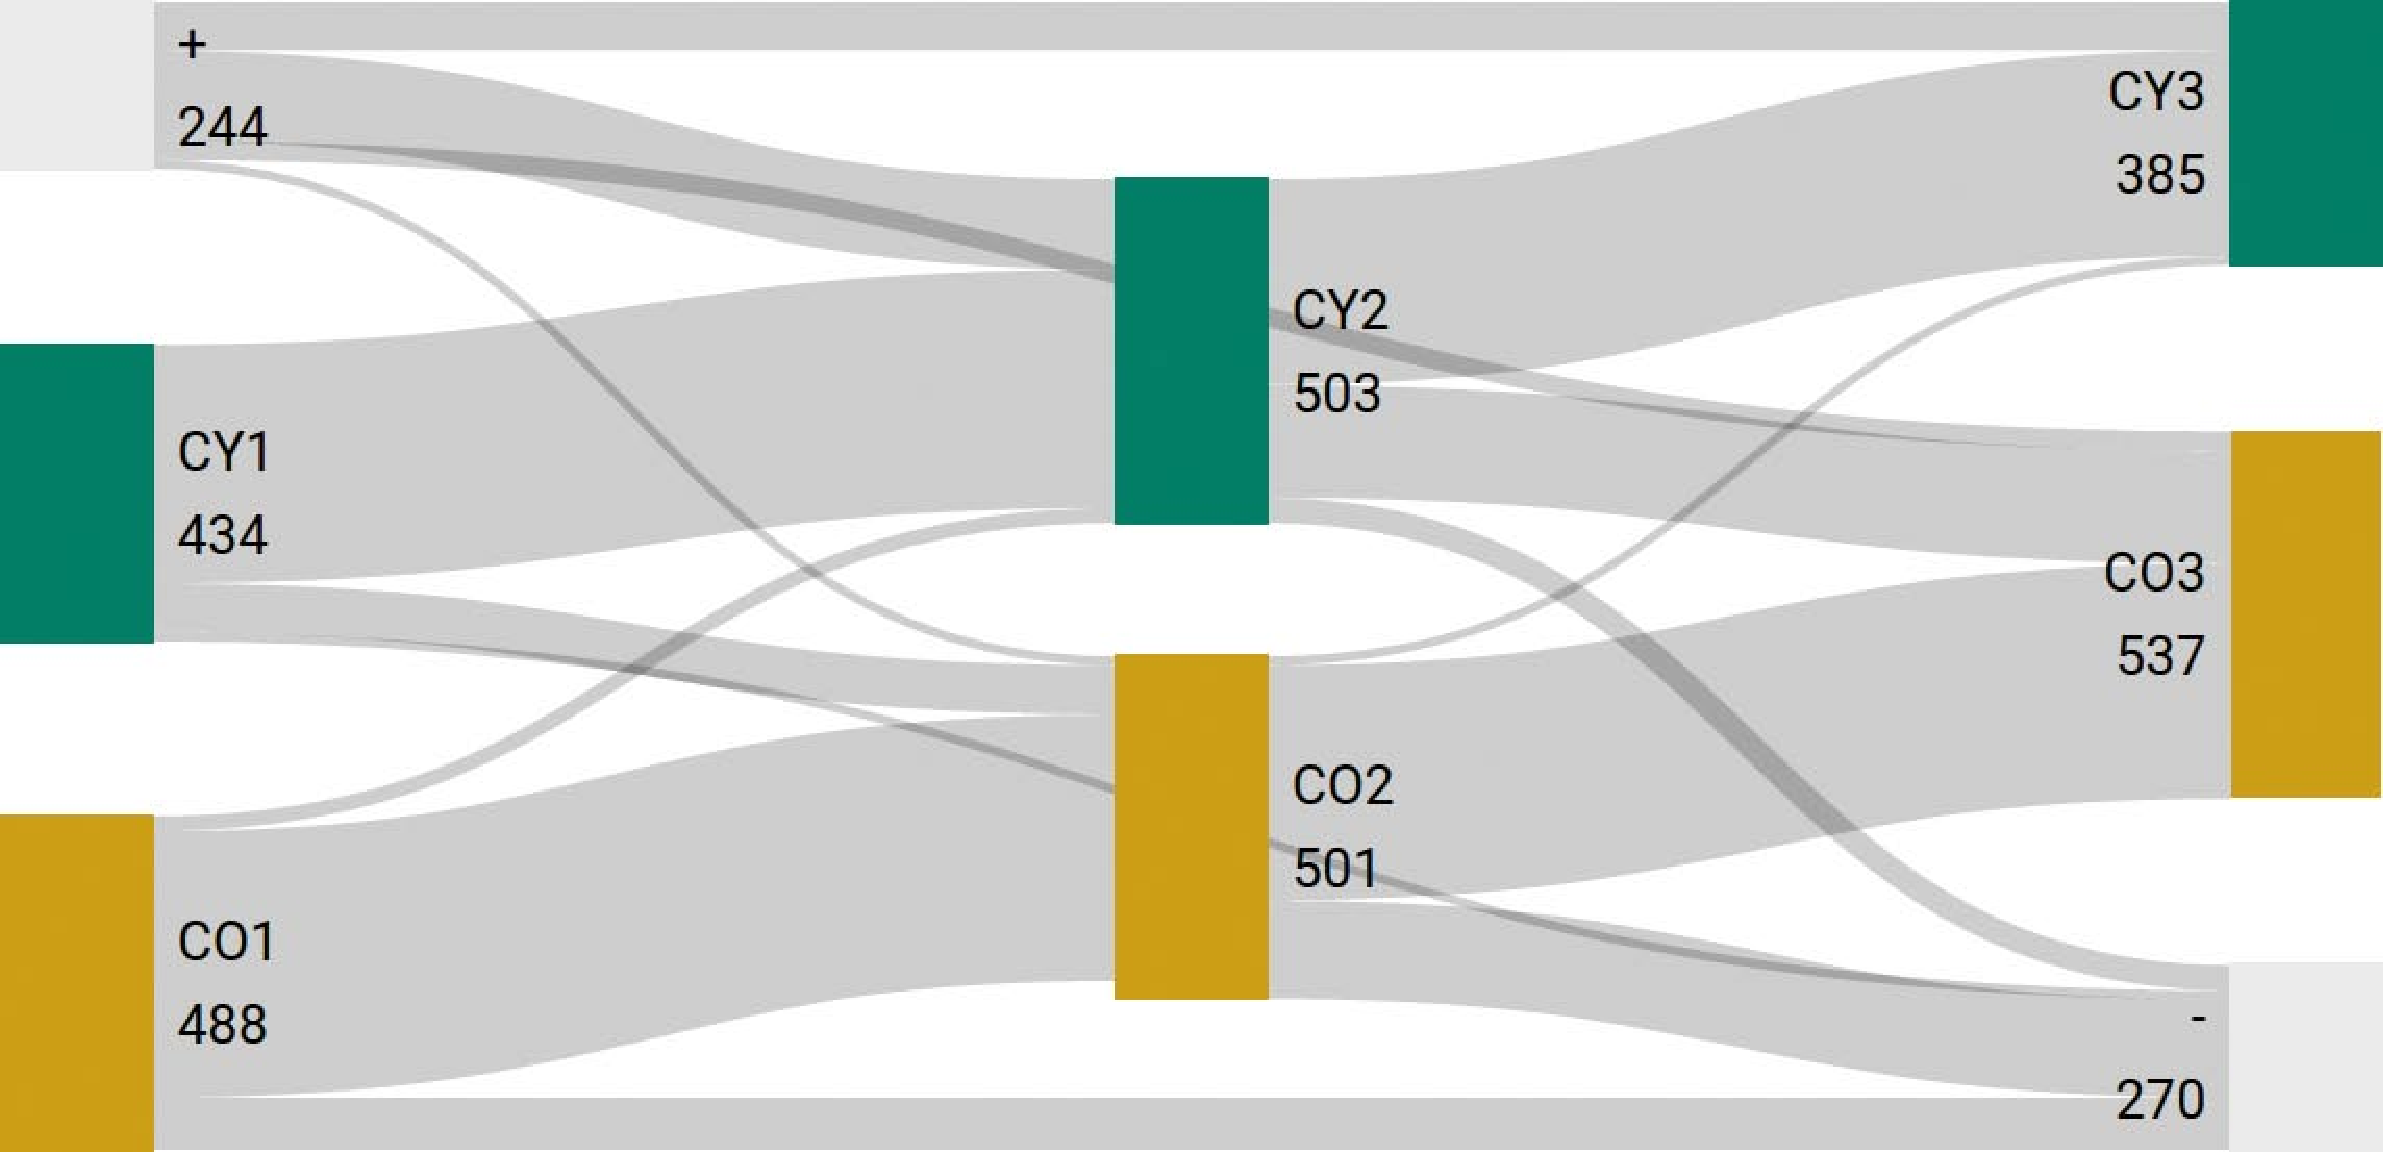
\includegraphics[width=1\textwidth]{Figures/LE_matching.pdf}
	\caption[Leading eigenvector (LE) communities]{Leading eigenvector (LE) communities}
	\label{fig:membersLE}
	\vspace*{10mm}
	\end{subfigure}
	\begin{subfigure}[b]{1\textwidth}
	\centering
	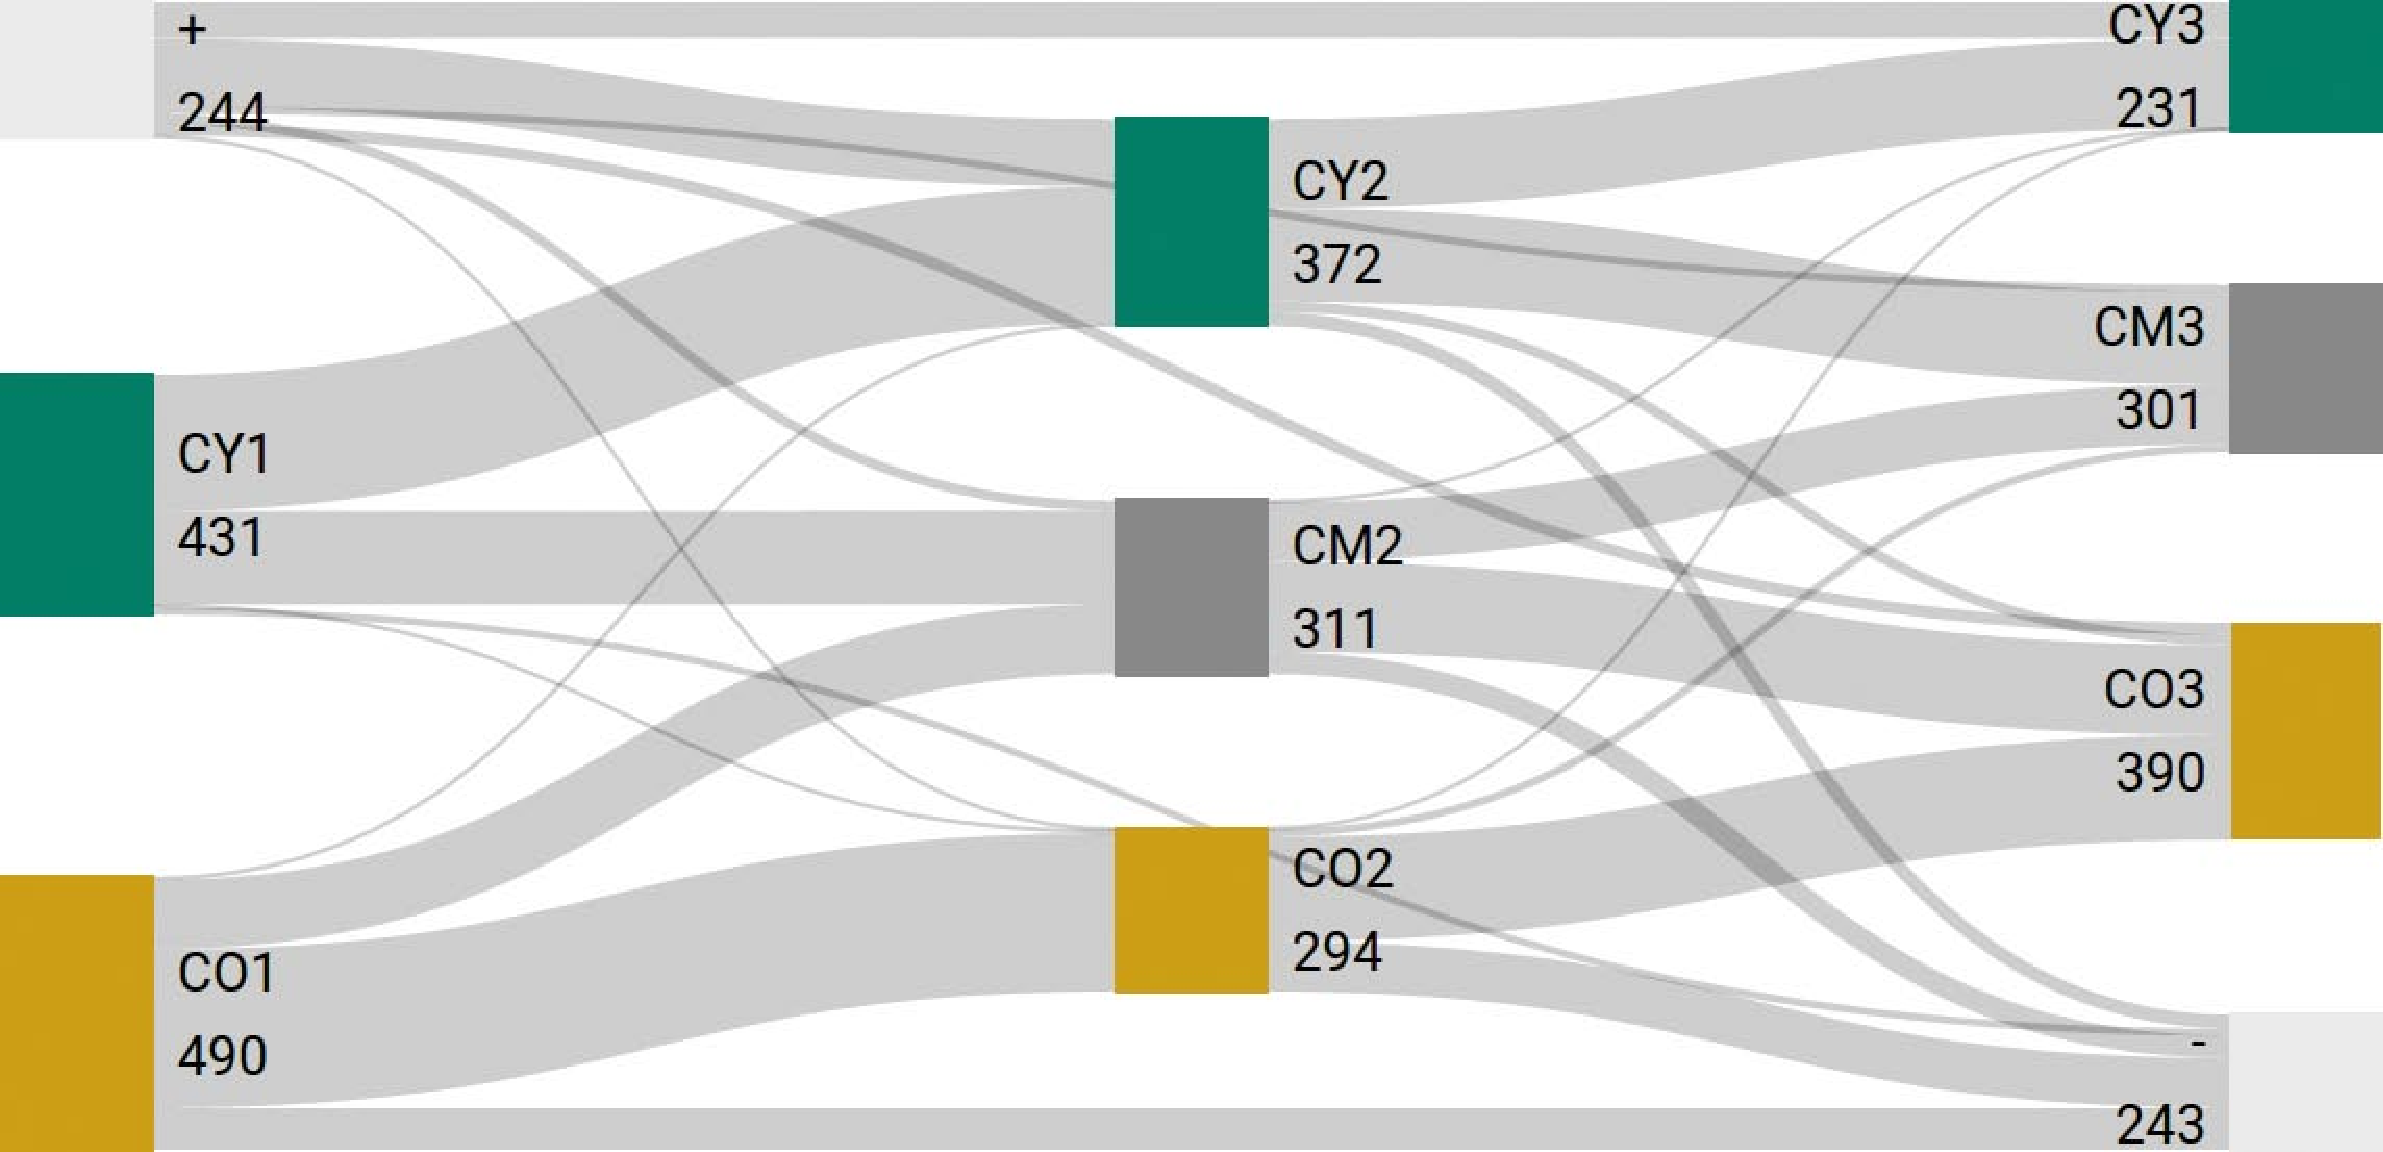
\includegraphics[width=1\textwidth]{Figures/WT_matching.pdf}
	\caption[Walktrap (WT) communities]{Walktrap (WT) communities}
	\label{fig:membersWT}
	\vspace*{5mm}
	\end{subfigure}
	\caption[Dynamics of bees]{\textbf{Dynamics of bees} 
	Each column represents a time step, the colored rectangles represent the communities for each step, and the height of the rectangles corresponds to the amount of its community members, as referenced by the number. \emph{Green} indicates the community containing young bees and the queen, \emph{gray} represents the community containing middle-aged bees (only for WT), and \emph{orange} the community containing old bees. This figure shows that the major part of the bees either stays in the same aged community or switches to an older group. The \emph{light gray} boxes represent the number of bees that are added to the colony and bees that disappear.}
	\label{fig:members}
\end{figure}
